%!TEX root = research_statement_yw.tex
%!TEX program = lualatex

\documentclass[10pt]{article}
\usepackage[
    top=0.5in,
    bottom=0.75in,
    left=0.5in,
    right=0.5in,
]{geometry}
\usepackage[
    protrusion=true,
    tracking=true,
    activate={true,nocompatibility},
    final,
    factor=1100]{microtype}
\SetTracking{encoding={*}, shape=sc}{40}

\usepackage{titling}
\setlength{\droptitle}{-4em}

\usepackage{fancyhdr}
\usepackage{lastpage}
\usepackage{xfrac}
\pagestyle{fancy}
\fancyhf{}
\renewcommand{\headrulewidth}{0pt}
\renewcommand{\footrulewidth}{0pt}

\usepackage{url}
\urlstyle{same}
\usepackage{wrapfig}
\usepackage[font=small,labelfont=bf]{caption}

\newcounter{fontsnotfound}
\newcommand{\checkfont}[1]{%
    \suppressfontnotfounderror=1%
    \font\x = "#1" at 10pt
    \selectfont
    \ifx\x\nullfont%
        \stepcounter{fontsnotfound}%
    \fi%
    \suppressfontnotfounderror=0%
}
\newcommand{\iffontsavailable}[3]{%
    \setcounter{fontsnotfound}{0}%
    \expandafter\forcsvlist\expandafter%
    \checkfont\expandafter{#1}%
    \ifnum\value{fontsnotfound}=0%
        #2%
    \else%
        #3%
    \fi%
}
\usepackage[T1]{fontenc}
% load babel here
\usepackage[no-math]{fontspec}
\usepackage[p,osf]{cochineal}
\usepackage[varqu,varl,var0]{inconsolata}
\usepackage[scale=.95,type1]{cabin}
\usepackage[cochineal,vvarbb]{newtxmath}
\usepackage[cal=boondoxo]{mathalfa}
\usepackage[scale=0.925]{FiraMono}
\iffontsavailable{JetBrains Mono, JetBrains Mono Italic}{%
\defaultfontfeatures{RawFeature={+axis={wght=400}}}%
\setmonofont[BoldFont={JetBrains Mono},%
BoldFeatures={RawFeature={+axis={wght=800}}},%
ItalicFont={JetBrains Mono Italic},%
BoldItalicFont={JetBrains Mono Italic},%
BoldItalicFeatures={RawFeature={+axis={wght=800}}},%
Contextuals=Alternate, Scale=0.925]{JetBrains Mono}%
}{}

\usepackage[inline]{enumitem}

% Dummy text
\usepackage{kantlipsum}

\usepackage{setspace}

% Absolute path
\usepackage{currfile-abspath}
\getmainfile % get real main file (can be different than jobname in some cases)
\getabspath{\themainfile} % or use \jobname.tex instead (not as safe)
\let\mainabsdir\theabsdir % save result away (macro will be overwritten by the next \getabspath
\let\mainabspath\theabspath % save result away (macro will be overwritten by the next \getabspath

\usepackage{cite}
\bibliographystyle{IEEEtran}

% Support IEEE BST control in non-IEEEtran document
\makeatletter
\def\bstctlcite{\@ifnextchar[{\@bstctlcite}{\@bstctlcite[@auxout]}}
\def\@bstctlcite[#1]#2{\@bsphack
    \@for\@citeb:=#2\do{%
        \edef\@citeb{\expandafter\@firstofone\@citeb}%
        \if@filesw\immediate\write\csname #1\endcsname{\string\citation{\@citeb}}\fi}%
    \@esphack}
\makeatother

\usepackage{xcolor}
\definecolor{link_col}{HTML}{5e81ac}
\usepackage[colorlinks=true, allcolors=link_col]{hyperref}

% Placeholder images
\usepackage{tikz}
\usetikzlibrary{patterns}
\usepackage[precision=2, unit=mm]{lengthconvert}
\newcommand{\dummyfigure}[3]{%
    \begin{tikzpicture}
        \draw [
            thick,
            pattern=north east lines,
            pattern color=black!10,
            inner sep=0,
        ]
        (0,0) rectangle (#1 - \pgflinewidth, #2 - \pgflinewidth)
        node[
                pos=0.5,
                align=center,
                font=\small,
                text width=#1,
            ] {
                #3 \\[2mm]
                \texttt{\tiny{Figure size: (\Convert{#1}, \Convert{#2})}}
            };
    \end{tikzpicture}%
}
%!TEX program = lualatex

\def\appPosition{Tenure-Track Assistant Professor}
\def\jobID{290722-FA}
\def\appDept{Department of Electrical and Computer Engineering}
\def\appSchool{University of Wisconsin-Madison}
\def\appAddr{%
    1415 Engineering Drive\\
    Madison, WI 53706%
}
\def\appArea{data-intensive computing}
\def\appSpecific{with significant implications for future computing systems, particularly bridging integrated silicon photonics, design automation, and hardware architectures for AI/machine learning applications} % for cover letter
\def\appCollab{silicon photonics, networked systems, computer architecture, design automation, and AI/machine learning}
\def\collabCustom{%
\emph{integrated photonics and optoelectronics} (Shubhra Pasayat, Chirag Gupta, Mikhail Kats, Zongfu Yu), \emph{VLSI design automation} (Azadeh Davoodi, Yu Hen Hu, Tsung-Wei (TW) Huang), \emph{computing architectures and systems} (Akhilesh Jaiswal, Mikko Lipasti, Umit Yusuf Ogras, Joshua San Miguel), and \emph{systems for AI/machine learning} (Kassem Fawaz, Younghyun Kim)%
}

%%%%%% Customize the following lines %%%%%%
\title{Research Statement}
\def\rsCustom{}
%%%%%% End of customization %%%%%%

\author{Yuyang Wang}
\date{\today}
\makeatletter
\fancyfoot[L]{\scshape \MakeLowercase{\@author}}
\fancyfoot[R]{{\scshape \MakeLowercase{\@title}}\quad{\LARGE\sfrac{\thepage}{\pageref*{LastPage}}}}
\makeatother

\begin{document}

\maketitle% this prints the handout title, author, and date
\thispagestyle{fancy}

In the dynamic landscape of distributed computing, the exponential growth in traffic demands within data centers and high-performance computing systems has been distinctive, fueled by a deluge of data-intensive workloads. This trend is prominently exemplified by the rapid expansion of machine learning, big data analytics, and most notably, deep learning (DL)\textendash driven artificial intelligence (AI) applications. The recent advent of large language models, which has revolutionized natural language processing and creative content generation, is propelling the broad adoption of ever-larger DL models and datasets, marking a significant milestone toward the era of data ubiquity. The continued scaling of these applications has pushed the limits of computational hardware, notably via increased parallelism and specialization. Yet, this rapid progress has outpaced the evolution of the underlying communication infrastructure, rendering chip-to-chip data movement a formidable barrier impeding performance and energy efficiency. This communication bottleneck has become the grand challenge to the quest of upscaling the computing systems toward exascale.

My research endeavors to find \textbf{transformative connectivity solutions}, maximally harnessing the potential of integrated silicon photonics (SiPh). In this pursuit, I have devised a dual-thrust research agenda for my independent career. The first thrust focuses on \textbf{reconfigurable system connectivity}. It aims to develop optical interconnects that not only provide unprecedented bandwidth but also adapt in real-time to the ever-evolving demands of emerging applications. The second thrust looks into \textbf{innovative system architectures}. It targets redefining chip-to-chip communication with groundbreaking optical I/O technologies, thereby pioneering new computational paradigms and interconnect functionalities. The synergy of these thrusts introduces unique design challenges, which I am equipped to tackle with my interdisciplinary research experience, ensuring the readiness of essential design tools and methodologies for these advanced connectivity solutions.

My research agenda is situated at the system level, squarely fitting into the interdisciplinary nexus of \appArea{} that bridges \appCollab{}. I look forward to the possibility of collaborating with the esteemed colleagues in the \appDept{} at the \appSchool{} to confront the grand challenge of data movement in future computing infrastructures across the full system stack.

\section{Research Accomplishments and Skills}
My doctoral and postdoctoral work have established a solid foundation for my anticipated research and equipped me with the skills necessary to address the upcoming research challenges. I was among the first to integrate accurate \textbf{compact models and simulation methodologies} of silicon photonic devices into widely used electronic design automation (EDA) platforms like Cadence Virtuoso~\cite{wuCompactModelingCircuitlevel2017,zhangCompactModelingSilicon2017}. This integration is crucial for the accurate co-simulation of electronic and photonic components, enabling the efficient development of complex photonic integrated circuits (PICs) with reliable performance estimation. My expertise in \textbf{process variation characterization, mitigation, and tolerance} ensures the robustness and energy efficiency of fabricated designs~\cite{wangCharacterizationApplicationsSpatial2020,wangEnergyEfficiencyYield2021,wangDispersionEngineeredFabricationRobustSOI2023}. This is particularly important for advanced technologies that often rely on emerging fabrication processes and require post-fabrication tuning. My work in these areas has been recognized in leading design automation conferences like DAC and ICCAD, respected photonics venues like OFC and JLT, and a forthcoming book chapter with Springer, effectively connecting the electronics and photonics research communities.

These design enabling techniques have been practically utilized in creating two generations of SiPh transceiver chips, featuring a \textbf{scalable link architecture} that facilitates unprecedented channel parallelism and delivers a chip I/O bandwidth of over 16 Tbps with energy consumption below 1\,pJ/b~\cite{wangScalableArchitectureSubpJ2023,wangCICC2024}. Fabricated in partnership with AIM Photonics through two full-wafer runs, each chip, measuring \textasciitilde{}70\,mm$^\text{2}$, densely integrates over 2,000 microresonators. The chip layout process was fully scripted and automated, showcasing not only significant technological advancements but also remarkable design efficiency. The highlighted link architecture was instrumental in securing a \$35M SRC JUMP 2.0 grant with 23 principal investigators, a program to which I have contributed through proposal writing and ongoing research efforts. This work has also resulted in invited papers and presentations at both photonics and electronics design conferences (Photonics West and CICC), and an invited journal submission to \emph{Nature Communications Physics}.

These accomplishments have advanced my research into exploring \textbf{traffic adaptability} for optical interconnects in distributed computing systems, grounding them in credible performance models and hardware validation. Notably, I have delved into runtime adjustments of parameters such as laser power and link bandwidth, aiming at accelerating distributed machine learning applications with reduced energy consumption~\cite{wangTaskMappingAssistedLaser2019,wangTrafficAdaptivePowerReconfiguration2021,brianJOCN}. A promising off-chip prototype, designed to redistribute wavelength channels across multiple ports at application runtime, is currently under review for publication. Additionally, an on-chip implementation is being fabricated at AIM Photonics and slated for testing in May 2024. These investigations underscore the significance of integrating architectural innovations and optimization strategies at the system level, a process which\textemdash without meticulous execution\textemdash could inadvertently counteract the advancements achieved at both device and link levels. This realization is a key driver behind my future research directions.

\begin{figure}[!t]
    \centering
    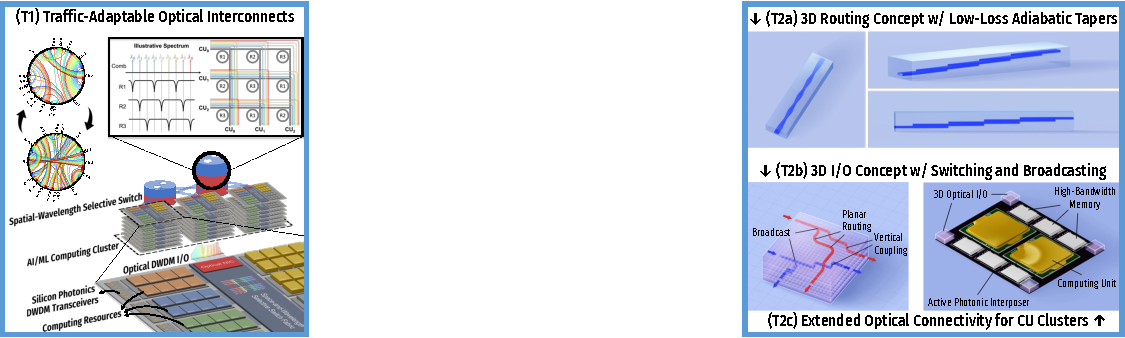
\includegraphics[width=\linewidth]{../../fig/research.pdf}
    \caption{Overview of my research background and future directions.}
    \label{fig:research}
\end{figure}

\section{Research Vision and Agenda}
% The need for high-bandwidth and energy-efficient connectivity is ubiquitous across all levels of network hierarchies. This necessity, coupled with the growing complexities arising from heterogeneous and dynamic traffic, calls for novel interconnect architectures that are not only high-performance but also versatile and adaptive.
My research agenda is set to continue at the system level, leveraging the latest breakthroughs in device designs and link architectures, while simultaneously informing their future advancements from a system application perspective. In light of the evolving data landscape, I plan to focus on two complementary and synergistic research thrusts in pursuit of groundbreaking connectivity solutions.

\subsection{Thrust 1: Reconfigurable System Connectivity}

With the advent of augmented reality (AR), virtual reality (VR), and Metaverse applications, distributed machine learning frameworks are seeing an increase in data privacy concerns that were previously confined to sectors with sensitive information, such as banking and healthcare. These sectors typically handle smaller volumes of data with more flexible latency requirements. In response, decentralized learning frameworks like federated learning have received growing popularity, as they allow the exchange of model parameters over raw data. Yet, certain applications still prioritize data parallelism to meet stringent requirements on model accuracy. Consequently, the data landscape in distributed computing is evolving toward both larger volumes and greater heterogeneity. This evolution, coinciding with the expansion of large models like GPTs, necessitates the next generation of optical interconnects to further excel in traffic adaptability, in addition to bandwidth and energy efficiency.

In this research thrust, my objective is to significantly enhance traffic adaptability by co-designing reconfigurable link architectures along with dynamic reconfiguration strategies. Building upon the SiPh transceiver developed during my postdoctoral research~\cite{wangScalableArchitectureSubpJ2023,wangCICC2024}\textemdash which stands out for its leading bandwidth capacity and energy efficiency among state-of-the-art solutions\textemdash I aim to incorporate greater reconfigurability into its design. My prior work, namely on runtime laser power scaling and link bandwidth reconfiguration~\cite{wangTaskMappingAssistedLaser2019,wangTrafficAdaptivePowerReconfiguration2021,brianJOCN}, serves as a proof-of-concept for the effectiveness of traffic-adaptable tuning knobs in improving both the performance and the energy efficiency of optically connected computing systems. Moving forward, I anticipate the success of this research thrust to be contingent on the following critical tasks:
\begin{enumerate}[nosep]
    \item Profiling and characterizing the traffic patterns of a diverse range of distributed computing applications, expected to exhibit greater heterogeneity and temporal dynamics compared to the collective communications typically observed in current computing clusters, as referenced in~\cite{brianJOCN}.
    \item Introducing additional reconfigurable parameters beyond laser power and link bandwidth, such as wavelength allocation and switching/routing, and developing runtime reconfiguration strategies tailored to these characterized traffic patterns.
    \item Conducting system-level simulations to assess the energy and performance impacts of the proposed reconfigurability, supported by credible performance models that accurately reflect real link designs.
    \item Designing and integrating reconfiguration modules with state-of-the-art SiPh transceiver implementations, and validating the enhanced interconnect architecture with reconfiguration strategies on a hardware testbed driven by realistic/production network traces.
\end{enumerate}
Throughout this endeavor, I also anticipate deriving valuable insights from a system application perspective. These insights will be instrumental in informing the design of SiPh devices and circuits, focusing on essential aspects such as tuning range and reconfiguration speed, to meet key performance metrics at the system level. This collaborative synergy across multiple design hierarchies is essential to maintain cutting-edge system connectivity in an ever-changing data landscape.


\subsection{Thrust 2: Innovative System Architectures}
Complementary to the first research thrust aimed at advancing chip-to-chip connectivity, the second thrust strives to address the notable gap between on-chip and off-chip communication bandwidths. This gap is particularly pronounced in accelerator systems comprising clusters of computing units (CUs) that frequently access data from both on-chip memory banks and off-chip memory pools. Expanding the number of on-chip high-bandwidth memory (HBM) stacks is increasingly impractical as the bandwidth capacity of electronic interposers approaches its limits. Conventional approaches using optical fibers to connect CU clusters and memory pools are also constrained by the size and pitch of fiber arrays. Nonetheless, the emerging concept of 3D optical I/Os, benefiting from dense waveguide routing across multiple layers, presents a promising avenue to scale up CU clusters with optical connectivity that stays on-board with extended reach. My contribution to assisting the formulation of this concept, which was successfully showcased at the 2023 DARPA ERI Summit, has inspired me to further explore this cutting-edge area. The key challenges I plan to address in this research thrust include:
\begin{enumerate}[nosep]
    \item Formulating the 3D routing problem with objectives such as maximized density and minimized loss, and developing efficient routing algorithms that draw from traditional EDA expertise and the latest in machine learning techniques.
    \item Informing the design of 3D routing elements with performance and area constraints, and optimizing their physical design employing recent advances in areas such as photonic inverse design and topology optimization.
    \item Conducting system-level design space explorations for computing architectures with transformed memory connectivity to delineate optimal system configurations, such as the ideal size of CU clusters that benefit from the expanded reach of on-board optical connectivity, and the optimal balance between on-chip and off-chip memory capacities.
\end{enumerate}
In addition to eliminating the bandwidth taper at chip boundaries and allowing for continued upscaling of CU clusters, this research thrust also promises to expand the role of optical interconnects beyond traditional data communication. For instance, certain computational tasks, such as matrix multiplication, can be offloaded to the optical domain, for which existing explorations have been limited by the vast difference in physical dimensions of electronic and photonic implementations. This limitation can be significantly alleviated by the manifolded density of optical components enabled by 3D routing. This thrust, therefore, not only addresses current technological limitations but also fosters the development of new computing paradigms, where optical interconnects assume a more dynamic and integral role in future computing system architectures.



\section{Research Collaborations and Initiatives}

My research experience has been deeply rooted in multidisciplinary collaboration, a skill I mastered during my postdoctoral training at the Columbia University. There, I led research initiatives within our group, guided by my supervisor's mentorship and backed by funding from agencies like DARPA, SRC, and ARPA-E. These initiatives required seamless teamwork with colleagues from academia, industry, and governmental bodies. In addition, I have a proven track record in assisting both my doctoral advisor and postdoctoral supervisor with fundraising activities. My responsibilities also encompassed preparing and compiling reports and materials, as well as participating in presentations at quarterly reviews to fulfill the requirements of our funded projects.

Given the interdisciplinary essence of my research agenda, I am enthusiastic about the opportunity to collaborate with the diverse faculty at the \appSchool{}. The expertise present in areas such as%
\rsCustom{}
\kant[7]

\footnotesize
\bibliography{\mainabsdir../../common/research_statement/bibliography}

\end{document}